\documentclass[a4paper,11pt]{article}%,twocolumn
\input{settings/packages}
\input{settings/page}
\input{settings/jupyter}
\usepackage[ framed, numbered]{matlab-prettifier}%framed,%
\usepackage{listings}
\usepackage{pdfpages}


\begin{document}
 
\begin{titlepage}
\center % Center everything on the page

%-------------------------------------------------------------------------------------
%	HEADING SECTIONS
%------------------------------------------------------------------------------------
\textbf{\large Department of Electronic and Telecommunication Engineering}\\[0.5cm]
\textbf{\Large University of Moratuwa, Sri Lanka}\\[1cm]
\textbf{\large EN2073 - Analog and Digital Communications}\\[2cm]
\includegraphics[width=0.3\textwidth]{figures/uomlogo}\\[2cm]

	
%-------------------------------------------------------------------------------------
%	TITLE SECTION
%------------------------------------------------------------------------------------
\textbf{\Huge Assignment 01 } \\[5cm]


%----------------------------------------------------------------------------------------
%	MEMBERS SECTION
%----------------------------------------------------------------------------------------


\vfill

\textbf{\large Submitted by}\\[0.5cm]

{\large Thalagala B.P.}	\hspace{5mm} {\large 180631J }\\[1cm]

%----------------------------------------------------------------------------------------
%	DATE SECTION
%----------------------------------------------------------------------------------------

\textbf{\large Submitted on}\\[0.5cm]
\textbf{\Large \today} % Date, change the \today to a set date if you want to be precise

%----------------------------------------------------------------------------------------

\vfill % Fill the rest of the page with whitespace
\begin{center}
	
	\textbf{\textit{ \large * {\tt MATLAB }Code used to generate the plots are attached at the end.}}
\end{center}

\end{titlepage}	



\section*{Q1: Plot of the signal $y(t) = A.cos(2.\pi.f.t)$}

\begin{figure}[!h]
	\centering
	\includegraphics[scale=0.45]{figures/q1}
	\caption{Plot of the signal $y(t) = A.cos(2.\pi.f.t)$, Where $A = 1$ and $f = 400 ~Hz$}
\end{figure}

\section*{Q2: Nyquist sampling frequency ($f_{nq}$)}

A function containing no frequency higher than $f$ Hz, is completely determined by sampling at $2f$ Hz. This frequency is called Nyquist rate or Nyquist sampling frequency.

\[\therefore Nyquist ~sampling ~frequency~of~above~signal = 2.f = 2\times400 = 800 ~Hz\]

\section*{Q3: Sampled signal at Nyquist sampling frequency ($f_{nq}$)}

\begin{figure}[!h]
	\centering
	\includegraphics[scale=0.45]{figures/q3}
	\caption{Sampled signal at Nyquist sampling frequency ($f_{nq} = 800 ~Hz$)}
\end{figure}

\section*{Q4: Sampled signal at ($2f_{nq}$), ($f_{nq}$) and ($f_{nq}/2$) }

For the given signal there is only one frequency component and therefore, there is no point in sampling it in the rate, higher than the Nyquist rate. Because of there are no other higher frequency components than 400 Hz,  signals sampled at both  $2f_{nq} = 1600 ~Hz$ and  $f_{nq} = 800~ Hz$ illustrated in top and middle subplots respectively, will be eventually reconstructed in to the same signal as there is \textbf{\textit{no contribution from the samples with zero amplitudes}} at the reconstruction stage.\\

Therefore, it will be good enough if we sample at the \textit{Nyquist frequency}($f_{nq} = 800~Hz$) as illustrated in the middle subplot and it is possible to reconstruct the original signal without loosing the important information.\\

Consider the signal sampled at the \textit{half of the Nyquist frequency}($f_{nq}/2 = 400~Hz$), that is the sampling rate is equal to the highest frequency of the signal and bottom subplot represents the effect of this. Because there is no change in the amplitudes of the samples it will be seen as a straight line or more accurately a sinusoidal with a lower frequency when we reconstruct the signal. Which indicates signal carries no useful information if we sample it in this frequency as we have lost all the higher frequency components and they are now seen as lower frequency components. This phenomenon is known as the ``\textbf{\textit{Aliasing or Spectral folding}}''.\\

\begin{figure}[!h]
	\centering
	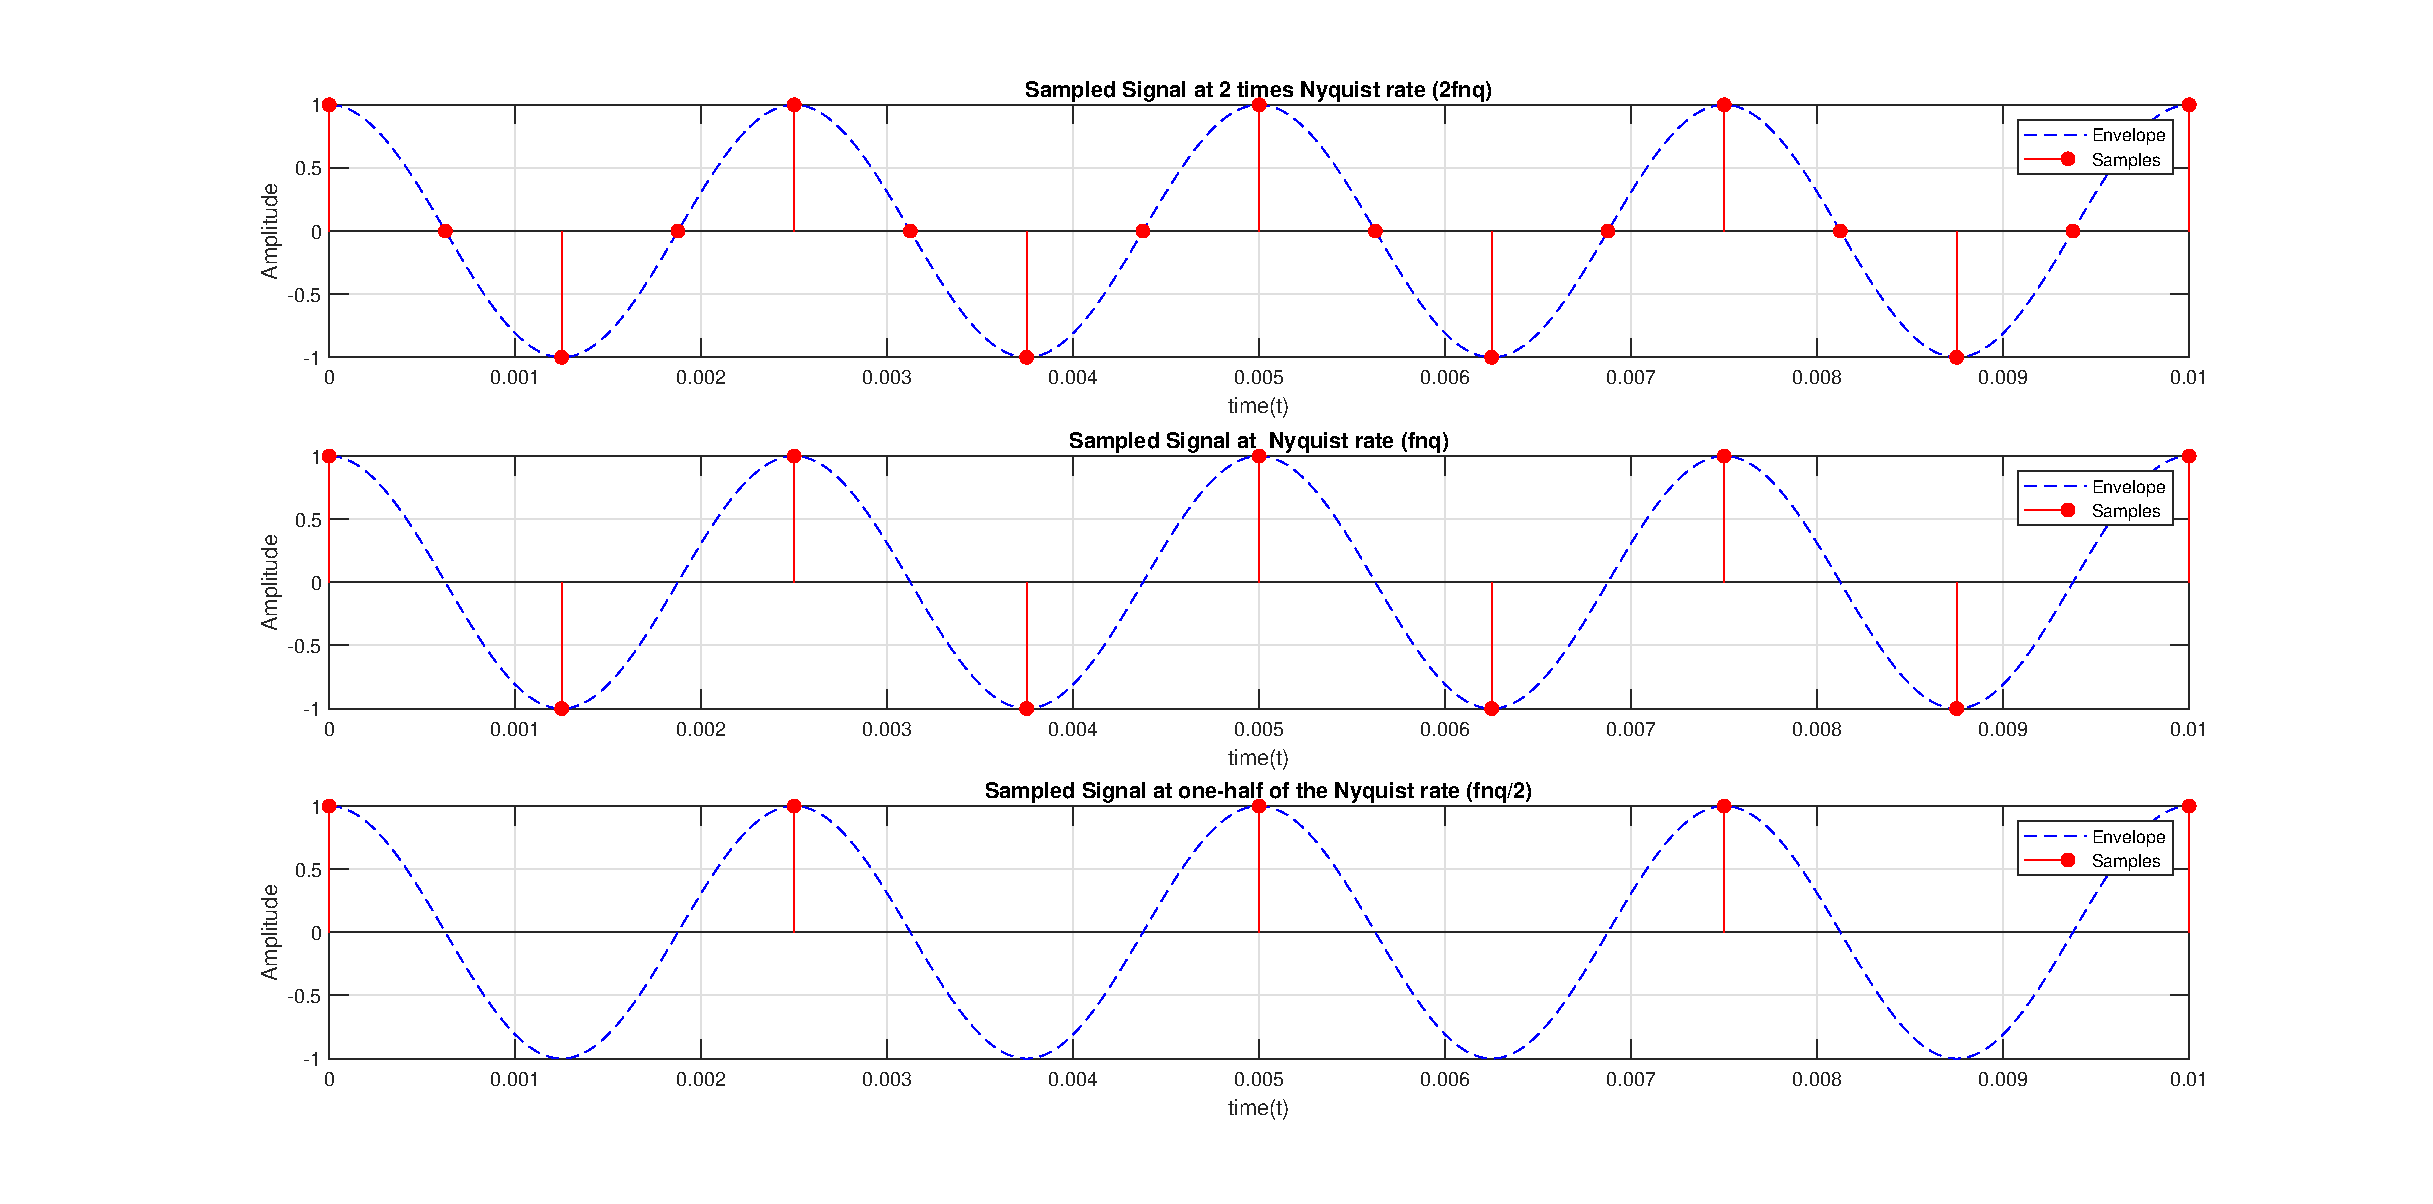
\includegraphics[scale=0.45]{figures/q4}
\end{figure}

\pagebreak
\section*{Q5: Minimum number of bits ($n_b$) required per a sample and number of minimum quantization levels (L) to have a $SN_qR$ ratio greater than 25dB}
 
$SN_qR$ in dB is defined as follows, where $S_0$ and $N_q$ represents the received signal power and the strength of noise power due to quantization.
\[
SN_qR = 10\log_{10}\left(\frac{S_0}{N_q}\right)
\]

Size of quantization interval can be written as follows \textit{for uniform quantization} where $L$ is the number of quantization levels and $m_p$ is the maximum amplitude of the signal. In our case which equals to 1.\\


\[Size ~of ~quantization ~interval~ (\Delta V) = \frac{2.m_p}{L}\]

Then $N_q$ and $S_0$ can be written as,
\[
\begin{split}
	S_0 &=\frac{m_p^2}{2}	
\end{split}
\hspace{1cm}
\begin{split}
	N_q &= \frac{\Delta V^2}{12}\\
	&= \frac{(2.m_p/L)^2}{12}\\
	& = \frac{m_p^2}{3L^2}
\end{split}
\hspace{1cm}
\therefore
\begin{split}
		SN_qR = 10\log_{10}\left(\frac{3L^2}{2}\right)
\end{split}
\]

According to the requirements following calculations can be done.

\[
\begin{split}
	SN_qR &= 10\log_{10}\left(\frac{3L^2}{2}\right)\\
	25 &< 10\log_{10}\left(\frac{3L^2}{2}\right)\\
	10^{2.5} &< \frac{3L^2}{2}\\
	\frac{10^{2.5}\times2}{3} &< L^2\\
	14.519 &< L
\end{split}
\hspace{2cm}
\therefore L_{min} = 16 ~(\because L~ must ~be~ a ~power ~of~ 2)
\]

Therefore number of minimum quantization levels (L) = 16 and  minimum number of bits ($n_b$) required per a sample is $\log_{2}(L) = \log_{2}(16) = 4$.

\pagebreak
\section*{Q6: Quantization of Sampled output values}

Following {\tt MATLAB} function implements a method to quantize a given sampled signal. Its functionality can be briefly described as follows.
\begin{enumerate}[]
	\item First the three special case of samples are considered.
	\begin{itemize}
		\item If the sample's amplitude equals to the maximum amplitude of the signal, then quantized value is set to be $m_p- \Delta V/2$.
		\item If the sample's amplitude equals to the minimum amplitude of the signal, then quantized value is set to be $m_p+ \Delta V/2$.
		\item If the sample's amplitude equals to zero, then there is nothing to quantize and the quantized value is set to be 0. 
	\end{itemize}
 	\item Then the other general values of the samples are considered. These values are again divided into two classes.
 	\begin{itemize}
 		\item If a sample is exactly equal to a value of a Quantization level, one of the following situations is possible and the quantization level is determined as follows with the aim of minimizing the effect of noise at the transmission.
 		\begin{itemize}
 			\item Negative samples are quantized towards negative infinity
 			\item Positive samples are quantized towards positive infinity
 		\end{itemize}
 		\item If a sample lies between two Quantization levels it is  quantized towards positive infinity.
 	\end{itemize}
\end{enumerate}
 


\lstinputlisting[basicstyle = \mlttfamily\scriptsize , style =
Matlab-editor]{code/quantizeSample.m}

\pagebreak
\section*{Q7: Quantization of the Signal sampled at 8 times Nyquist rate ($8f_{nq}$) with 16 Quantization Levels}

Observe the following figures while paying attention to the grids which makes it easy to identify the change in amplitudes after the quantization. Corresponding  Sampled Values and Quantized Values are also given below and it is seen that both {\tt 1.0000  and  0.9239} are quantized on to the {\tt 0.9375} quantization level and other values are quantized onto the corresponding discrete levels.

\begin{verbatim}
Sampled Values:	
1.0000    0.9239    0.7071    0.3827    0.0000   -0.3827   -0.7071   -0.9239   -1.0000
Quantized Values:
	0.9375    0.9375    0.6875    0.4375         0   -0.4375   -0.6875   -0.9375   -0.9375
\end{verbatim}

\begin{figure}[!h]
	\centering
	\includegraphics[scale=0.45]{figures/q71}
	\caption{Sampled Signal at 8 times Nyquist rate ($8f_{nq}$)}
\end{figure}

\begin{figure}[!h]
	\centering
	\includegraphics[scale=0.45]{figures/q72}
		\caption{Quantization of the Signal sampled at 8 times Nyquist rate with 16 Quantization Levels}
		\label{l16}
\end{figure}

\pagebreak
\section*{Q8: Quantization of the Signal sampled at 8 times Nyquist rate ($8f_{nq}$) with 32 and 8 Quantization Levels}

\begin{verbatim}
Sampled Values:		
	1.0000    0.9239    0.7071    0.3827    0.0000   -0.3827   -0.7071   -0.9239   -1.0000
Quantized Values:	
0.9688    0.9063    0.7188    0.4063         0   -0.4063   -0.7188   -0.9063   -0.9688
	
\end{verbatim}

\begin{figure}[!h]
	\centering
	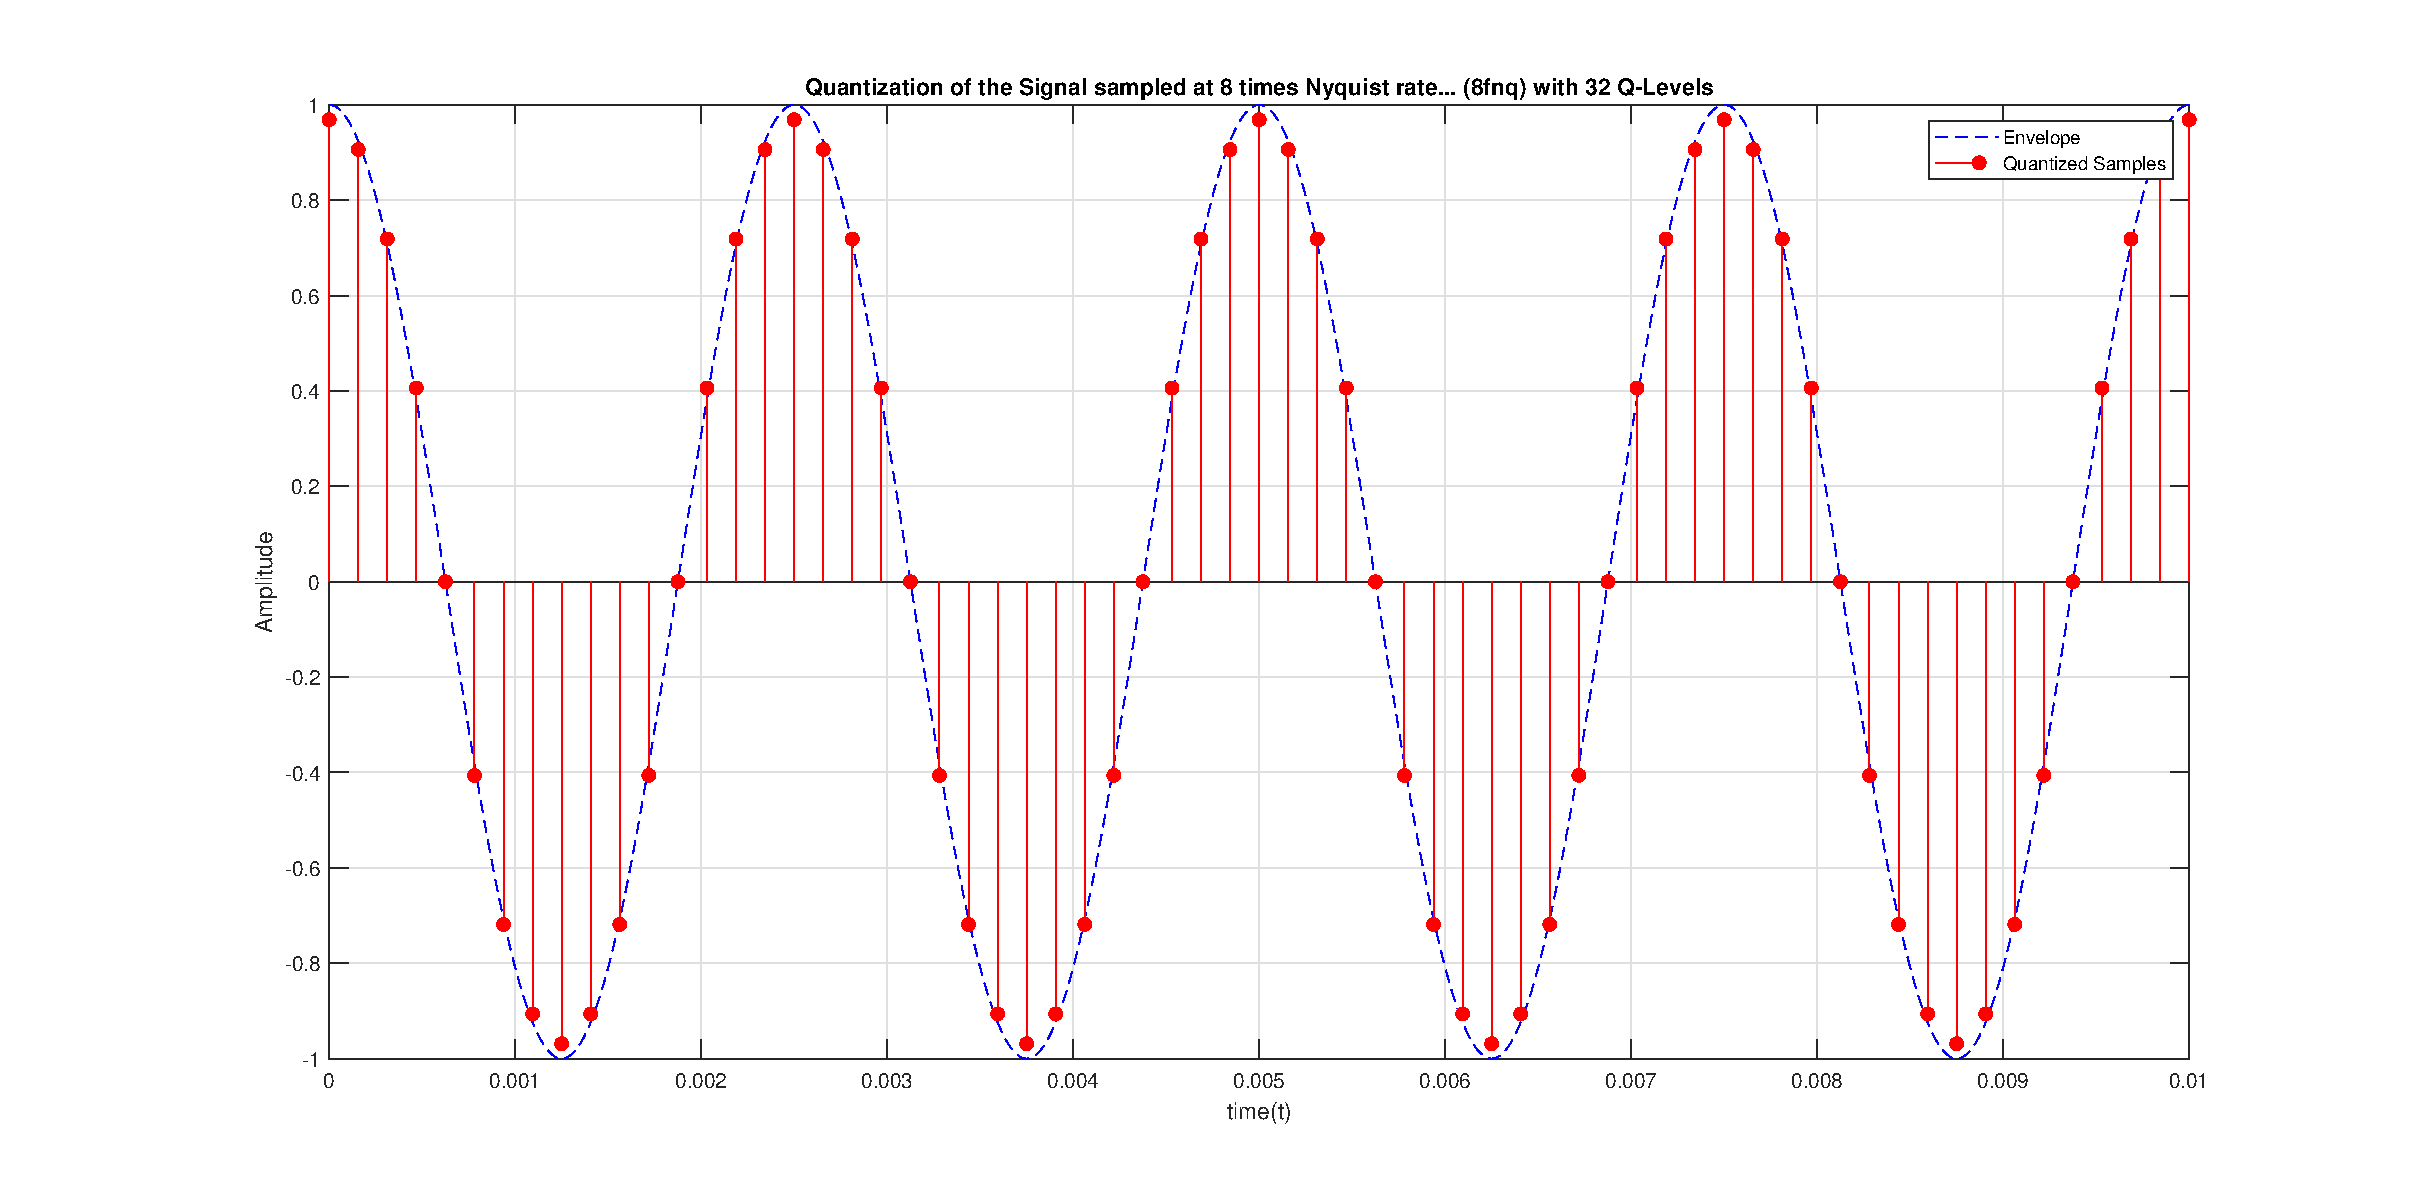
\includegraphics[scale=0.42]{figures/q32l}
	\caption{Quantization of the Signal sampled at 8 times Nyquist rate with 32 Quantization Levels}
	\label{l32}
\end{figure}

\begin{verbatim}
Sampled Values:		
	1.0000    0.9239    0.7071    0.3827    0.0000   -0.3827   -0.7071   -0.9239   -1.0000
Quantized Values:	
	0.8750    0.8750    0.6250    0.3750         0   -0.3750   -0.6250   -0.8750   -0.8750
\end{verbatim}
\begin{figure}[!h]
	\centering
	\includegraphics[scale=0.42]{figures/q8l}
		\caption{Quantization of the Signal sampled at 8 times Nyquist rate with 8 Quantization Levels}
		\label{l8}
\end{figure}

\pagebreak

\begin{verbatim}
	Sampled Values:		
	1.0000    0.9239    0.7071    0.3827    0.0000   -0.3827   -0.7071   -0.9239   -1.0000
	
	Quantized Values with 32 Levels:	
	0.9688    0.9063    0.7188    0.4063         0   -0.4063   -0.7188   -0.9063   -0.9688	
	
	Quantized Values with 16 Levels:
	0.9375    0.9375    0.6875    0.4375         0   -0.4375   -0.6875   -0.9375   -0.9375
	
	Quantized Values with 8 Levels:	
	0.8750    0.8750    0.6250    0.3750         0   -0.3750   -0.6250   -0.8750   -0.8750
\end{verbatim}
\vspace{1cm}
When observing the above plots and the given values  following conclusions can be made.\\ 

\begin{itemize}
	\item As depicted in Fig. \ref{l32} when the quantization levels are increases every sampled value is mapped into a unique quantization level but when we decrease the number of quantization levels as in Fig. \ref{l16} and Fig. \ref{l8} several sample values may be mapped into the same quantization level. This introduces an ambiguity at the signal reconstruction stage as we have lost the information about actual value of the amplitudes.
	
	\item In  addition to that when the number of quantization levels are decreased the actual value of the sampled signal and the value of the quantized signal differs a lot which again introduces an ambiguity at the signal reconstruction stage. This can be clearly seen when comparing the original signal's envelope drawn in dashed line with the quantized signal.
\end{itemize}

Therefore in order to minimize the quantization noise we need to increase the number of quantization levels.
 

%\vfill
%\hrule
%\begin{center}
%	Executable code for this assignment can be found  \href{https://github.com/bimalka98/Computer-Vision-and-Image-Processing/blob/main/EN2550Assignments/A2/180631J_a02.ipynb}{here}.
%\end{center}
  
\includepdf[pages=-]{code.pdf}
  
\end{document}
